\chapter{Datenbl�tter}\index{Datenbl�tter}


\textcolor{darkred}{Anmerkung: Wenn das Thema der Diplomarbeit auch Hardware-Komponenten bzw. den Aufbau eines Demonstrators eingeschlossen hat, so ist ein Anhang mit den wichtigsten Datenbl�ttern sehr sinnvoll. Zum Einen k�nnen interessierte Leser direkt ohne Internetrecherche die Betriebsparameter der Komponenten einsehen, zum Anderen ist somit auch eine gute Dokumentation des Systems f�r die Bedienung durch andere Anwender als den Autor gegeben. Auch wenn die Datenbl�tter normalerweise online verf�gbar sind, so erspart der beigef�gter Anhang dem Anwender eine aufw�ndige Recherche. Die Anzahl Seiten sollte 25--30 nicht �berschreiten.}

\textcolor{darkred}{Genau wie bei den Quelltextabschnitten im Anhang muss aber auch bei den Datenbl�ttern ein kurzer Abschnitt vorweg geschickt werden, welcher die Auswahl der Datenbl�tter und die Relevanz erkl�rt.}

\textcolor{darkred}{Die einzuf�genden Datenbl�tter sollten im pdf-Dateiformat vorliegen und nicht als Grafik, sondern als ganze Seite einzuf�gen.}


Die nachfolgenden Datenbl�tter erl�utern Systemparameter, Funktionsweise, Anschlussvarianten und Betriebsarten zu dem im Rahmen der vorliegenden Arbeit verwendeten Maxon-Motorregler ADS\_E 50-10.



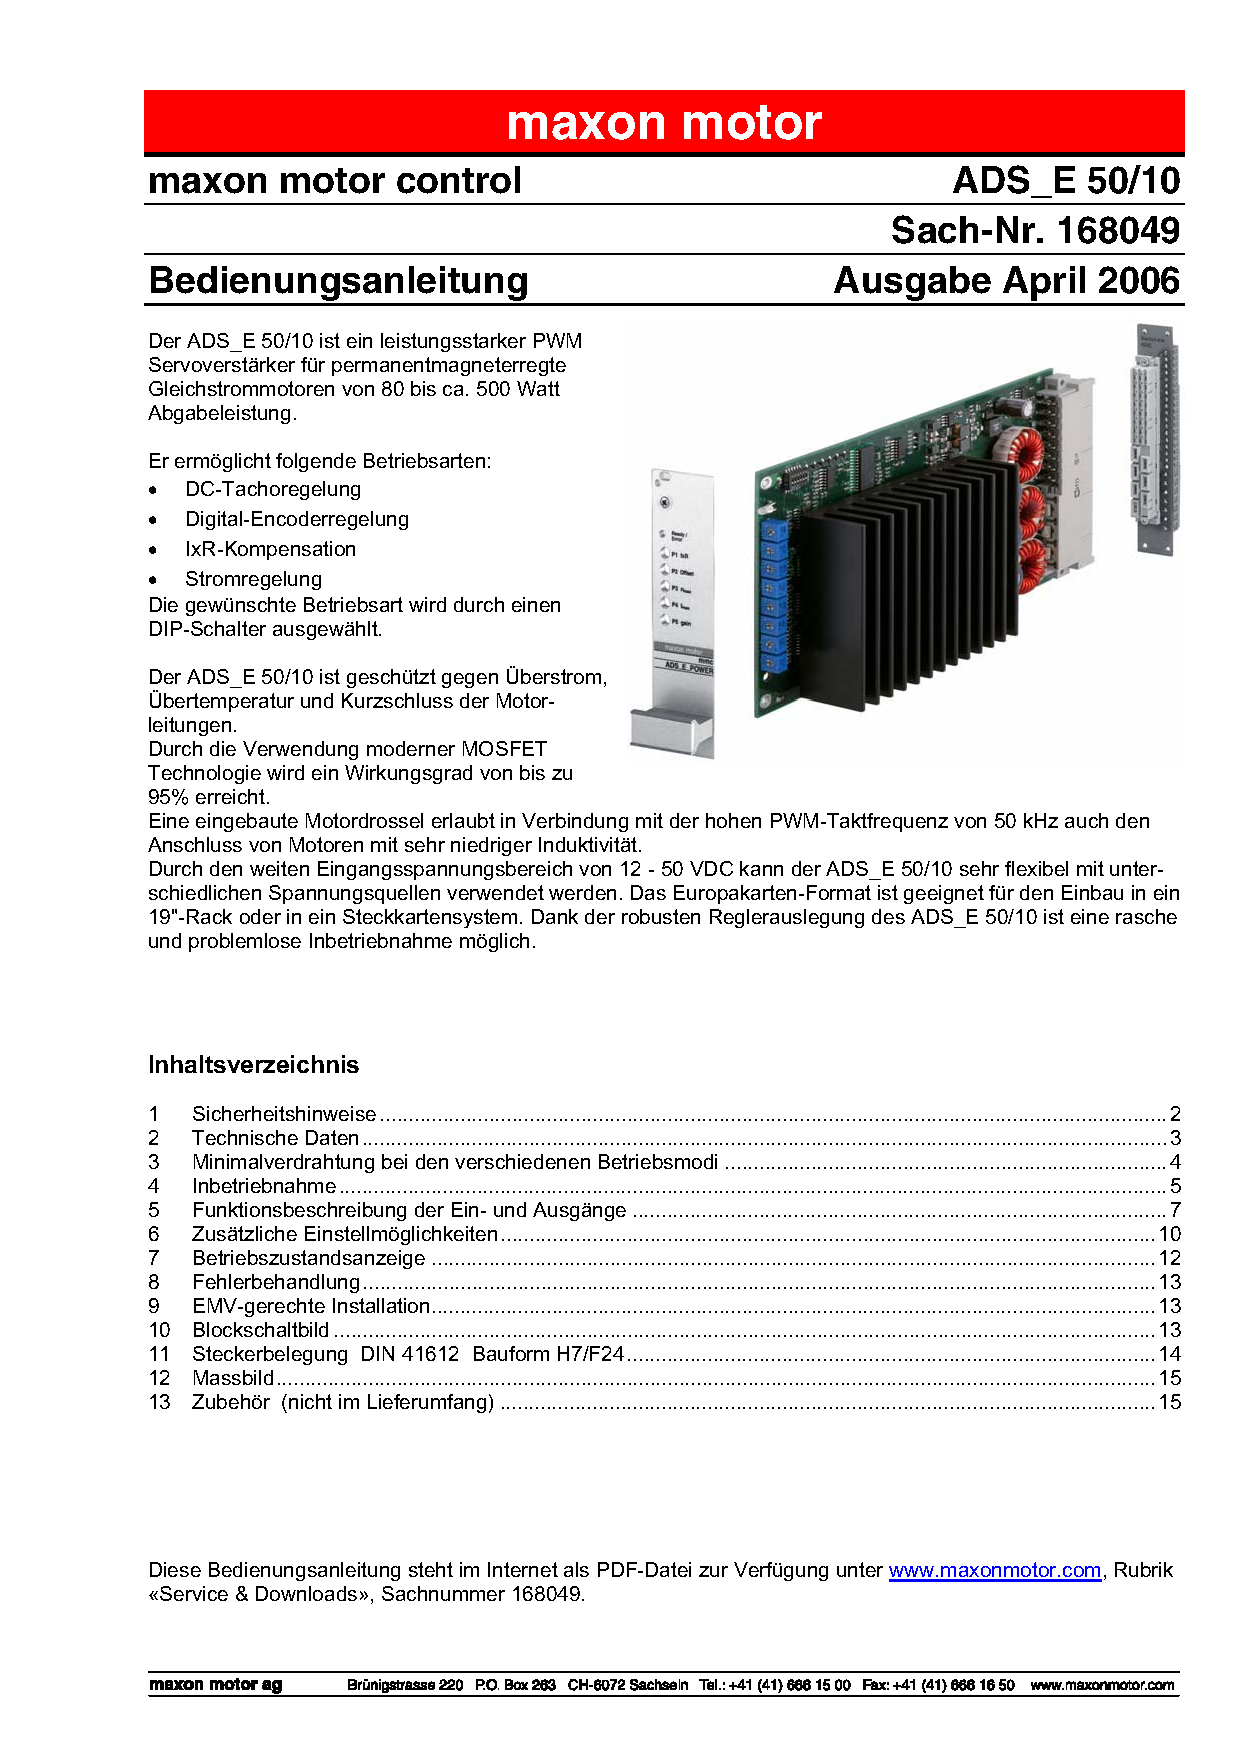
\includepdf[
   pages={-},
   nup=1x1,
   landscape=false,
   noautoscale=false,
   turn=false,
   scale=0.8,
   trim= 0mm 0mm 0mm 0mm,
   clip=true,
   pagecommand={},
   delta=0mm 0mm
]{BilderAnhangD/Seiten_aus_ads_e50_10_de.pdf}

%
% Vorsicht: Pfad- und Dateiname darf keine Leerzeichen enthalten
%

